\documentclass[11pt]{article}
\usepackage[top=1.00in, bottom=1.0in, left=1.1in, right=1.1in]{geometry}
\renewcommand{\baselinestretch}{1}
\usepackage{graphicx}
\usepackage{natbib}
\usepackage{amsmath}
\usepackage{hyperref}
\usepackage{todonotes}

\def\labelitemi{--}


\begin{document}
\bibliographystyle{/Users/Lizzie/Documents/EndnoteRelated/Bibtex/styles/besjournals}
\renewcommand{\refname}{\CHead{}}

\title{Effects of phenology on plant community assembly and structure }
\author{Elsa E. Cleland* \& E. M. Wolkovich*}
\date{\today}
\maketitle
\tableofcontents


\setlength{\parindent}{0cm}
\setlength{\parskip}{5pt}
*Authors contributed equally.

% One figure idea below (on traits), but really want on contrasting life histories

\section{Text in need of a home}

\emph{Definition to fit in ...} 
% timing of recurring growth and reproductive events (Ackerly)
% Isabelle is more of the `timing of recurring life history events ilk' and she stressed the seasonality of phenology as needing to be in the definition, but then we discussed tropical phenology etc. and she came around to this.
We define phenology as the timing of critical stages of growth and reproduction and the transitions between them. This definition is intentionally more inclusive than some other definitions, which focus on recurring or seasonal events, and thus can narrow phenology to only certain plant types or biomes (e.g., woody species in the temperate zone). We find this narrowing artificial and think it can limit a broader understanding the selective pressures on phenology that---as we outline below---are critical for understanding the role of phenology in community assembly. Our definition thus includes both tree leafout, and seed germination of annual plants at the same time in encompasses fruiting, flowering and importation transitions in and out of these phases, such as dormancy and vernalization (see potential figure idea \ref{fig:phenologycircles}).

Phenological `events' are rarely one moment in time ... we could get into distributions and plasticity here... (Or leave it where I have it below?)

\emph{Text on frost and other traits ...} 
In many systems, spring frost is likely a controller on phenology that could lead to trait correlations. In most temperate and boreal systems freezing temperatures limit growth throughout part of the year, shaping the spring phenology of most species. Leafing or flowering before the last spring frost can mean losing tissue, but simply pushing all phenological events well after frost has its own costs as it means higher competition for light and other resources. 

This temporal landscape of shifting frost risk and competition predicts early species should have traits that allow them to cope with frost, but be competitively inferior under low resource conditions, while later species should show the reverse. Recent reviews suggest some evidence for this \citep{wolkovich2014aob,memegan2021}, but few have directly tested traits related to frost tolerance and avoidance, possibly because of the diversity of ways early-active species can deal with frost \citep{frostbook}. Species vary in what temperatures can cause tissue damage \citep{Lenz2013}, but universally tissues are most vulnerable during budburst and leafout \citep{frostbook,vitasse2014earlier,cat2019}, thus species often have a suite of other mechanisms including waxy or hairy leaves to slow ice formation, rapid budburst to speed through the most dangerous period or cheap-to-build tissues so that tissue lost can be quickly replaced \citep{frostbook}. This last mechanism fits neatly with a competition trade-off as leaf and vessel tissues that are easy to build are also those that generally cannot compete well under low resource conditions \citep{larcher1980,diaz2016global}. 

\section{Main text}

\emph{Introduction} 

Phenology, defined here as the timing of growth and reproductive events, is a key plant trait because it is often closely tied to the fitness of individuals in seasonal environments \citep{verdu2005early,munguia2011meta}. The timing of phenological transitions determines both the environmental conditions and biotic interactions experienced by individuals during different stages of their life-cycles \citep{donohue2005niche}, and hence the relative impact of these factors on survival and reproduction \citep{caruso2019meta}. For instance, in temperate ecosystems, the timing of leaf emergence or flowering in spring can determine fitness consequences of frost events \citep{inouye2008effects,augspurger2013reconstructing}, or the impacts of herbivores \citep{meineke2021phenological}, on plant performance.

Plant phenology has also garnered global attention because observations suggest that phenology of many plant species has shifted in recent decades, associated with rising temperatures and co-occurring global changes \citep{wolkovich2012warming,parmesan2015plants,menzel2020climate}. In response to experimental warming, plants generally display earlier spring events (e.g. leaf-out, flowering) and later fall events (e.g. senescence) \citep{stuble2021plant}. However, there is considerable variation among species in their phenological sensitivity to both observed and experimental warming \citep{cook2012divergent,wolkovich2012warming}. Species that track climate change by having greater plasticity for accelerated early-season phenology have been found to maintain or even increase their performance in experimental settings \citep{cleland2012phenological,wolkovich2021phenological}. Hence, species-level phenological responses to global changes have the potential to influence process at the population- \citep{iler2021demographic}, community- \citep{cook2012divergent,caradonna2014shifts}, and ecosystem-scales \citep{piao2019plant} .

Phenology is one of many interacting traits that influence the suitability of an organism to its environment. Functional traits are at the core of many theories in community ecology (with the key exception of neutral theories, e.g. \citet{hubbell2005neutral}, especially those aiming to predict the assembly of local communities from a larger regional species pool. It is often assumed that plants have a suite of traits that determine their ability to survive and reproduce in different environments \citep{schimper1902plant}, and that traits also reflect strategies of resource-capture, such that species with similar traits will compete, leading to competitive exclusion during community assembly \citep{gause1932experimental,macarthur1967limiting,abrams1983theory}. Despite the recognized importance of phenology for understanding species responses to the environment, and structuring species interactions in communities, phenology is missing from many frameworks seeking to identify major axes of global plant trait variation (e.g. \citet{westoby1998leaf,wright2004worldwide,diaz2016global,joswig2022climatic}. Yet, it is recognized that phenology is essential in trait-based approaches to understanding species interactions and community assembly \citep{cope2022role}.

Here we focus our review on the role that phenology plays in plant community assembly. We examine how phenology enters into major theories of community assembly, including the potential for phenology to influence competitive and facilitative interactions, and to shape priority effects. We also examine the role that phenology plays in life- history trade-offs, and how phenology shapes species co-existence. In addition to reviewing the theory, we review studies that document community assembly following disturbance, shifting community composition in response to global environmental changes, and the role that phenology plays in invasion by exotic species into resident communities, including efforts to assemble native communities that are resistant to invasion through restoration. We consider the role of multiple phenological transitions, including germination or seedling emergence, bud-burst or leaf-out, flowering, seed maturation and dispersal, and senescence.
%maybe change "life-history trade-offs" to "ecological trade-offs", and take out dispersal and seed maturation unless we actually address their phenology?

Although evolutionary responses of phenology to changing conditions could play an important role in community assembly (e.g. \citet{cavender2019diversification}, we focus our review on ecological studies. To maintain our focus on community assembly, we have not included studies that focus on single species, nor on purely ecosystem-level measures of phenology. While trophic mismatch \citep{kharouba2018global} is a potential outcome of shifting species phenology in response to global change, it is beyond the scope of this review. We also will not discuss how multiple global change factors interact to influence phenology (e.g. \citet{zhou2023climate}, nor the specific cues that underlie phenological transitions (e.g. \citet{chuine2017process}. Although we may not yet understand the mechanisms by which different factors interact to influence plant phenology, the principles are well-discussed elsewhere.

\subsection*{Phenological assembly: From the abiotic to biotic environments} % Section 2

Communities assemble from a pool of potential species through a series of abiotic and biotic sorting processes \citep{hillerislambers2012rethinking}. At the largest scale, a community's assemblage is limited by species present in a wider regional pool---species well suited to an environment will thus not occur in any one local community unless they are present in this regional pool. From this pool, species are filtered based on the abiotic environmental conditions of a particular location---species must be able to persist through a local environment's extremes in hot, cold, dry, wet and other factors to pass through this `environmental filtering' step of assembly. This collection of potential species that could form a community is then filtered once more---by the now smaller, local pool of species itself \citep{hillerislambers2012rethinking}. 

Competitive, facilitative, predatory and all other biotic interactions determine which species together can co-occur in the long term. If two species compete too strongly, then only the stronger competitor will remain in the local community at this step. Similarly obligate mutualists, predators and parasites will persist only if the other species they require are present in the community. This final stage of assembly is where much of community ecology has focused over its history as a subdiscipline, driving theories of coexistence, including whether species even truly `coexist' or merely are on a slow walk to extinction for all but one species in each community \citep{Hubbell:2001vo}. 

Phenology enters community assembly at both the environmental (abiotic) and biotic filtering steps. Species phenologies must match the environment to pass the first filter: their growth and reproduction must be timed to match periods when the environment is mild and resource-rich enough for these events. Thus, in an environment with cold sub-freezing winters, species generally must have well-timed dormancy to avoid growing too much in the middle of the winter when they would lose new tissue. Similarly, arid and tropical environments impose filters against certain phenologies. Once a set of species passes the environmental filter, phenology matters again at the biotic filtering step, where species with too similar phenologies may compete too strongly to co-occur.  Alternatively, species that overlap phenologically have the opportunity to develop facilitative interactions \citep{duchenne2021phenological} promoting co-occurrence, while species with little phenological overlap are unlikely to interact via biotic filtering processes.

These two steps at which phenology is relevant to community assembly suggest a simple temporal matching that obscures the underlying complexity of most phenological `events,' such as leafout or fruiting. First, while `event' suggest an almost instantaneous timepoint, this is gross simplification. Phenology is an attempt to extract and simplify the temporal dimensions of various developmental processes that can rarely (if ever) be one point in time. Instead, phenology is generally a series of distributions. For any one event within one individual, there is a distribution of the process starting, peaking and ending, which can be variously imagined as a normal curve or sigmoid curve (imagine the event of a grape cluster ripening: the number of berries ripening each day mapped over time, would look normal, while the progress towards all berries ripened would be sigmoid, potential Fig.  \ref{fig:histsigmoid}). This then scales up across individuals within a population, and across populations \citep{inouye2019}. Such complexity is generally simplified into an `event' that often represents the 50\% point extracted statistically after repeated observations. 

Second, phenology---as a point in time---can appear highly flexible or strongly fixed---depending on how time is defined. To date, much work has used calendar time for phenology: a snowdrop flowers on a certain day of the month in one year, for example, and on another day another year. When measured this way, phenology appears highly flexible---jumping around in temporal space from year to year or place to place---as the environment is variously warm, cool, dry or wet. Yet, plant phenology can also appear highly deterministic when defined in biological time; that is, when defined as relative to a set of known environmental triggers, such as accumulated cool temperatures known to vernalize some flowering species. When the underlying triggers or cues for phenological events are fairly well understood for some events (with perhaps flowering in \emph{Arabidopsis thaliana} being the best understood) phenology can be highly predictable and effectively---inflexible. For the purposes of our review here, we cotton more to the latter interpretation which strips away complexities of geography that do not necessarily aid our understanding of phenology \citep{davies2013}. 

\emph{Where phenology fits in the environmental vs. biotic filtering part of community assembly}
% Check out Kraft thought piece (separating out biotic and env is almost impossible, focus on tolerance; in FuncEco), but also ask JD 

The importance of phenology to species passing the environmental filter of community assembly has been long studied---though rarely framed in exactly these terms. Early studies of the controls on species ranges stressed phenology as a major axis \citep{salisbury1926geographical}. Today process-based models based almost entirely on species phenology are highly predictive of tree species ranges \citep[where they have been tested,][]{chuineJTB,Morin:2009gt,morin2007}. These models integrate over both growth and reproduction: trees in temperate systems leafout, flower and fruit then lose tissue to frost if temperatures dip below their cold limits (which vary for leaves, flowers and fruit), they then must have a long enough season for fruit development. Various species along various range edges are limited by tissue damage, fruit ripening or carbon starvation---depending on the summed outcome of a phenological model \citep{Chuine:2010gm}. 

Range models based on phenology highlight the life history challenges of phenology---species must fit in a sequence of events to grow and reproduce within environmentally feasible periods. Through this lens, the sequence and length of phenological events becomes critical, and prevalent trade-offs from life-history theory become more relevant. For example, trade-offs between fruit size and time available to grow (growing season length) may drive some species to flower before they leaf \citep{dan2021nph}. Similarly, trade-offs between growth, reproduction and survival may determine how often an individual invests in reproduction \citep{schaffer1974optimal,law1979cost,stearns1998evolution}. These complexities are present in many process-based models, but rarely extend beyond into either life history or community ecology theories. Process-based models similarly view phenology often as a static trait that shapes broad-scale (biogeographical) processes \citep{Chuine:2010gm}, with little focus on the role it may play within communities. Yet plant invasions suggest this view is overly narrow.

Recent work on plant invasions suggest a role for phenology beyond environmental filtering and instead through biotic assembly mechanisms \citep{wolkovich2011phenology,Fridley:2012fj}. Theory in invasion biology focuses both on the characteristics of the species invading, and on the community into which it invades, with the vacant niche model proposing that species should invade if there is open `space' in a community and the invader fits that space. Phenologically, this predicts species not to simply filter in based on their phenological match to the abiotic environment, but on their match to the biotic environment. Invaders should thus take advantage of open temporal space within communities, which some evidence suggests they do---particularly at the start and end of seasons (see next section). 

Findings from invasion biology support a potential role of temporal niches more broadly in community assembly \citep{gotelli1996}. Static environments (e.g., a chemostat) cannot easily support temporal niches, but even slightly more complex dynamics of resource availability across a season can create the potential for temporal niches (Fig. \ref{fig:resource}). Models including a simple resource pulse that starts a growing season can theoretically create space for temporal niches and thus phenological assembly (discussed further in the section on coexistence). Such models, however, highly simplify the resource dynamics of most environments, which is more aptly described a multi-dimensional mosaic of access to light, water, and nutrients variously present through abiotic factors (weather, tree fall due to storms etc.) and lost through uptake and use by other species. This complexity leaves much room for the order of species arrival to matter.

\subsection*{Priority effects}

In addition to the roles of environmental filtering and biotic interactions for determining the temporal niches of species in assembled community, the relative timing of arrival of a species can influence community assembly through priority effects \citep{alford1985priority,chase2003community,fukami2015historical}. Priority effects have often been considered as historical contingencies in the process of community assembly, arising from the chance establishment of individuals of different species, resulting in different community compositions across sites that are otherwise similar in terms of species pools, environmental conditions and disturbance histories \citep[e.g.][]{diamond1975assembly}. In the context of succession, early studies noted that the timing of disturbance relative to seasonality of seed dispersal could result in different species initially colonizing sites, and variation in later species abundances \citep{keever1950causes,holt1972effect}. More recently, it has been recognized that the relative order of species’ growth onset throughout the growing season can also greatly influence the relative abundance of species later in the season via priority effects \citep{fukami2015historical,wainwright2012seasonal,rudolf2019role}.  Phenology is a key aspect of a species niche, and hence should be key to niche-based predictions of community assembly \citep{vannette2014historical}.

The predictive power of priority effects for understanding community assembly suggests that the potential for competitive exclusion is not even across the growing season, and should drive patterns where phenologically earlier species are competitively dominant. For instance, the timing of germination is a trait which is highly linked to plant fitness, because it determines both the biotic and abiotic environment experienced by the emerging seedling \citep{donohue2010germination}. Foundational studies demonstrated that earlier germinating individuals achieved higher adult size, likely via space and resource preemption, and competitive suppression of later germinating individuals of the same species \citep{ross1972occupation},  a type of asymmetric competition \citep{connolly1996asymmetric}. Subsequent work has found repeatedly that earlier germinating species gain a competitive advantage over later germinating species \citep{cleland2015priority,waterton2016trade,blackford2020species}. Hence it is unsurprising that seeds can “sense” the presence of neighboring seeds, and display accelerated germination in more competitive environments \citep{dyer2000accelerated}.

However, a number of factors can reduce the benefit of early germination phenology. For instance, apparency to herbivores \citep{waterton2016trade} or exposure to sub-optimal conditions such as early-season drought \citep{wainwright2012seasonal} can create trade-offs whereby later germinating species can achieve numerical dominance. Further, priority effects are not always competitive; experimental work with \textit{A. thaliana} has shown that individuals germinating during stressful periods of the growing season can be facilitated by neighbors \citep{leverett2017germination}. This finding is broadly consistent with the prediction that competitive priority effects will be stronger under conditions of high resource availability or low stress \citep{vannette2014historical}, opening the door for facilitative priority effects to arise under stressful conditions.

Priority effects arising via differential germination timing are likely to be most important in herbaceous-dominated ecosystems, but may also arise in woody-dominated ecosystems via the timing of spring green-up, due to light preemption by species with earlier growth dynamics. For instance, the non-native Amur honeysuckle (\textit{Lonicera maackii}) invades the understory of deciduous forests in the Eastern U.S., where it has earlier leaf-out in the spring likely associated with greater frost tolerance compared with co-occurring native shrubs \citep{mcewan2009leaf}. The potential for priority effects to arise directly from earlier season flowering are less clear mechanistically, and early-flowering species are more prone to frost damage in temperature ecosystems \citep{inouye2008effects}. However, the timing of flowering can be indicate of the timing of soil resource uptake, with important implications for community assembly \citet{gulmon1983phenology},\citet{seabloom2003invasion}.

Restoring native plant communities, and preventing invasion by exotic species, are two areas where phenological priority effects can play a key role in optimizing desired endpoints of community composition. Non-native species have sometimes been observed to germinate \citep{wainwright2012seasonal,wilsey2011biodiversity,marushia2010phenology} or flower \citep{cleland2013strengthening} earlier than co-occurring native species, suggesting phenological priority effects may be one factor predicting the successful establishment of invaders into resident communities \citep{wolkovich2011phenology,alexander2019earlier}. Mechanistically, earlier phenology may allow invaders to avoid competition by exploiting a vacant phenological niche, or window of opportunity \citep{gioria2014resource}. Or, priority effects can also be mediated by plant-soil feedbacks whereby earlier active invaders can change the environmental conditions for later active native species \citep{grman2010within}. However, other reviews have found that phenological differences between invading and resident species differ across regions \citep{godoy2009flowering} or found limited evidence of phenological differences between native and non-native species \citep{zettlemoyer2022limited}. There have also been cases where later-active invaders that achieve greater size outcompete early-active native species \citep{godoy2014}. Together these findings suggest that the role of phenology in invasion inherently depends on how phenology correlates with other traits important for community assembly.

In the context of restoration, introducing target native plants to a recently disturbed site either earlier in the season, or as larger plants rather than seeds, can give them a priority advantage over invasive species in the seedbank \citep{young2017using,wilsey2021restoration}. Experimental studies sometimes find that phenological priority effects of invasive species are stronger under conditions of nutrient enrichment \citep{kardol2013resource,valliere2022phenological}  consistent with theoretical predictions \citep{vannette2014historical}.  Restoration strategies can help reduce the seasonal priority effects of invading species on native communities, for example reducing nutrient availability through carbon additions, or planting early-active native species \citep{cleland2013strengthening,hess2019priority}. Additionally, early-season exposure to herbivores \citep{waterton2016trade} or early-season herbicide treatments (\cite{marushia2010phenology} could aid restoration goals by reducing priority effects of invading species.

Climatic context is also likely to pay a role in phenological priority effects. Inter-annual climate variation \citep{levine2011seasonal}, or directional changes in climate, can change the relative order of species seasonal phenology or the correspondence of temperature and moisture cues (\cite{kimball2010contemporary}, resulting in altered species interactions and species relative abundances \citep{thomson2017between,kimball2010contemporary,buonaiuto2023contrasting}. Thus, seasonal priority effects will likely play a key role in understanding changing species compositions in plant communities with future climate change.

\subsection*{Phenological coexistence}

By defining the temporal niche, phenology links clearly to theories of species coexistence focused on niche partitioning. Decades of theory have posited that plant communities are organized by a final critical filter where each species uses a unique set of temporal, spatial and otherwise environmental resources \citep{Hutchinson:1959xi}, which may be shaped in part by predators and mutualists \citep{mcpeek2022coexistence}. This allows each species to be uniquely superior in one particular $n$-dimensional niche space and thus increases intra-specific competition above inter-specific competition---a critical component for species to coexist \citep{Chesson:2000vd,hillerislambers2012rethinking,mcpeek2022coexistence}. Through differing vegetative phenologies, species could use similar resources but occupy distinct temporal niches and thus coexist. 

Coexistence through niche differences is often referred to as a `stabilizing mechanism' in the canon of what is now often called `modern coexistence theory' \citep{Chesson:2000vd}. This theory divides mechanisms of this final stage of community assembly into stabilizing mechanisms---which increase intra-specific competition relative to inter-specific and thus can contribute to coexistence through species differences---and equalizing mechanisms---which decrease fitness differences. Equalizing mechanisms generally reduce true coexistence, but can lead to apparent coexistence as two identical species will generally co-occur in nature for a very long time  \citep[until one is lost to stochasticity,][]{Hubbell:2001vo}. This canon has dominated coexistence research of recent decades and underpins recent work to integrate phenology.

A number of recent studies leverage niche differences to argue that phenology is critical to coexistence in plant communities. \citet{godoy2014} found that differences in phenology tended to increase niche differences in experimentally assembled grassland communities of native and exotic species, but this did not promote coexistence. Instead, the phenological uniqueness of some invaders promoted their invasion, while other invaders benefited from an apparent correlation between phenology and competitive ability (later active species---both native and exotic---appeared competitively superior to early-active species). Correlated phenology and competition was also used by \citet{rudolf2019role} to insert phenology into classical coexistence equations for competing species. In this approach, increased phenological differences between competitors promote coexistence when the earlier species is the inferior competitor. \citet{memegan2021} apply a similar trade-off to show that a species attribute strongly related to phenology---`environmental tracking'---can be critical to coexistence when it trades off with how well species convert resources to new biomass. Most recently \citet{levine2022competition} added phenology to classical coexistence equations by allowing species to have longer or shorter seasons; here coexistence is possible if phenology trades-off with a growth rate advantage---effectively a type of competitive advantage.  

As these studies highlight, recent research heralding the importance of phenology to coexistence all leverage a similar trade-off between phenology and competitive ability. Given the domination of competition in current coexistence theory and research \citep{mcpeek2022coexistence}, this seems the most obvious and natural point to insert phenology into coexistence. Superficially the idea that phenology and competition trade-off is very attractive: if species vary their overlap in time, they should compete less and reduced interspecific competition should increase stabilizing niche differences and promote coexistence---but this is not the exact angle these models are leveraging. Instead they posit that earlier or later species (depending on the model) are competitively superior (through one parameter or another) thus invoking a rather simple trade-off. This trade-off would work equally well for many plant traits; fundamentally any plant trait added to a classic competition model such that it trades off with competitive ability will promote coexistence through stabilizing niche differences. Our current insights into how phenology specifically effects coexistence is thus, still rather narrow and not terribly specific to phenology. 

These models also generally insert phenology as a coexistence mechanism mostly independent of environmental variation---even though phenology itself varies year to year with environmental variation. These current studies, like much of the work on modern coexistence theory focus on resource partitioning---a fluctuation-independent mechanism of coexistence---ignoring an additional suite of likely relevant mechanisms that are fluctuation dependent: relative non-linearity of competition and the storage effect. While not yet tackled (to our knowledge) and certainly more complex to model and study, these two mechanisms seem highly relevant to phenology. Relative non-linearity promotes coexistence through variation in competitive intensity over time or space, given that species have different nonlinear responses to competition \citep{CHESSON:1994vn,Chesson:2000vd}. Recent work suggests relative non-linearity may be an important and under-appreciated mechanism in plant communities, but attempted to `control' for phenology rather than consider it \citep{hallett2019rainfall}. Yet species varying phenologies could produce varying competitive intensity over time and/or create the required non-linear response for coexistence via relative non-linearity. 

% [And they're missing the fun meat ... ] While most recent work on modern coexistence theory focuses on separating stabilizing and equalizing mechanisms, the theory also encompasses and overview of the three ways coexistence can occur: relative non-linearity, XX and the storage effect. 
% From Chesson 2000 'In the case of temporal fluctuations, these mechanisms can be divided into two broad classes: relative nonlinearity of competition and the storage effect.' and the other is mean fitness differences (according to my notes from working with Megan way back when).  You can check out: https://eeb.arizona.edu/chesson-lab which has links for fluctuation dependent (links to resource partitioning) and fluctuation independent mechanisms, which is handy. 
Similarly, the underlying mechanisms of storage effect---where species vary in their responses to the environment, and that response covaries with competition---could clearly relate to phenology, as is often theoretically proposed \citep{Chesson:1993gi,Chesson:2004eo}, but rarely tested. Instead the storage effect today is generally tested on interannual timescales for annual plants, where the model prediction that species `store' environmentally favorable periods (`buffered population growth') can be tested through seedset. Older work focused on storage outside of seedbanks, however, has made phenological predictions. \citet{Kubo:1996qe} generated a model of coexistence for tropical forest trees where species compete for spatial gaps---and their associated resources---at the start of climatically favorable periods each year. The model predicted phenological diversity across tree species that depended both on the length of climatically unfavorable periods and the phenological widths of species---effectively the size of the temporal niches \citep{Kubo:1996qe}. Storage occurred through long-lived adult stages, with seedbanks assumed to have weak dormancy (and thus could not provide `storage' of good environments). This approach contrasts in the method of storage compared to models today focused on annual plant communities, yet both approaches have similarly allowed storage through only one mechanism and focused on inter-annual timescales.

Yet the complexity of species phenologies and overall life histories makes it seems likely they may use more diverse timescales and multiple types of `storage'. (Just the way chinstrap penguins get in a good night's sleep through thousands of daily micronaps....)  Indeed the definition of `storage' in the storage effect model highlights this complexity---and unites varying life histories under one model---storage can be through seed banks, long-lived life stages in perennials, or through dormancy periods \citep{Chesson:2000vd}. Most plant communities contain a mix of these storage strategies across species, and within species multiple ways to store environmentally favorable periods seem common. Including this complexity in coexistence theory, however, likely requires modeling phenology as a more nuanced and complex trait. % and dealing with the complexity and constraints of time ....

% And maybe something here on that they're missing predators and disease? ... 

\subsection*{Limited time within seasons and lifespans} % Putting the life history back in the timing of plant life history events

Phenology captures a major axis of how organisms deal with limited time. Time is inherently limited for all organisms---both each season and over their lifetimes---by abiotic and biotic drivers that shape each organism's schedule of growth and reproduction. Most of the literature on phenology focuses on the annual schedule---events that occur and often recur each year---but the lifetime schedule also matters \citep{post2008phenological,park2022seasonal}. Integrating this lifetime perspective, however, requires bridging to life history theory, which has worked to predict the optimal schedule of growth and reproductive timing across an organism's lifetime, generally ignoring finer scales within lifetimes, where many phenological events fall \citep[but see][]{ejsmond2010time}. Each field has thus focused on its own version of time---phenology on the seasonal or annual version and life history theory on the lifetime version---in part because of the challenge of integrating across them. Integrating across these temporal perspectives is critical, we argue, since each is likely to impact the other. %:  the lifetime schedule strongly impacts the annual schedule, and vice versa. 

% Phenological events are often treated today as though they are independent, but they never are ...
Integrating across timescales highlights that phenological events are non-independent in ways critical for understanding phenology. All single phenological events are part of a larger schedule, constrained in multiple ways. First, most growing seasons have climatically unfavorable periods for growth that make time a limited---and bounded---resource. Plants need to grow and reproduce within these bounds while dealing with a second major constraint---certain immovable sequences. A fruit cannot occur without flowering and leaves cannot senesce before they start growth. These combined constraints create a geometric optimality problem well-suited to life-history theory, but---we argue---one that may also be imperative to solve for useful advances in phenological community assembly.

Much current research in the role of phenology within plant community assembly treats phenological events as independent. Empirical work on trade-offs focuses generally on only one event and often one part of the season (e.g., spring leafout). Similarly, models of the role of phenology in coexistence generally simplify phenology to a single trait---though what event or events this links to is rarely clear \citep[even when studied with empirical data][]{godoy2014}. Because phenology generally trades-off with resource competition in most models, events related to growth such as germination, or leafout seem likely candidates for some models \citep[e.g.,][]{godoy2014,memegan2021}, but others seem to implicitly model phenology as total growing period \citep{levine2022competition}. Most accurate to these models would be when resource uptake is greatest, which recent research suggests relates to phenology \citep{Heberling2013,heberling2019}, but perhaps not in ways that allow us to generalize from phenology to resource uptake across species. Further, most models appear to ignore reproductive events, such as flowering and fruiting, which occur before leafout for many species \citep{Primack:1987jz,dan2021nph} and may play a large role in determining the timing of growth events \citep{ettinger2018phenological}. The complexity of this only increases when integrating over how the timing of fruit development relates to the timing of pollination and seed dispersal, both of which also appear under strong selection \citep{whitehead1969wind}.


This current focus in plant phenological assembly on growth events, with little mention of reproduction, seems to miss increasing evidence that reproductive phenology is as or more important than growth phenology. While life history theory generally predicts growth before reproduction, many plants flower before they leaf, with research suggesting this is driven by strong selection on flowering \citep{dan2021nph} . Studies of full sequences of phenological events within a year---including growth and reproduction---find little evidence that leafout or senescence (growth events) affect flowering or fruiting, but strong evidence that the development time of fruit may constrain senescence and other growth events \citep{ettinger2018phenological}. Current studies of trade-offs focused on growth-related phenological events may thus miss where selection is potentially acting on the trade-offs, and highlight the problem of simplifying a constrained sequence to a single unconstrained and independent event. Better recognizing and integrating phenological sequences could solve part of this problem, but doing so usefully will require more efforts to develop models and theory across timescales. 

% Is it actually phenology that matters in these coexistence models, or is it investment choices?
Integrating across intra- and inter-annual timescales is a common---and challenging---topic in both community assembly and life history theories. Most work generally focuses on one temporal scale or the other but plants clearly integrate risk and reward across these scales, leading to diverging lifespans, growing season lengths and fundamental strategies that likely operate within and across years. Building up to understand this requires models that incorporate storage alongside growth and reproduction. Earlier work in this area suggested maximizing reproduction given growth and storage across unfavorable climatic periods replicated the relative timing of leaf growth and senescence for broad classes of species, suggesting diverging plant strategies depending on the productivity, stability and reliability of the habitat \citep{iwasa1989optimal}. More recently this area of life history theory has been focused on capital breeding animals \citep[e.g.,][]{varpe2009adaptive}, but provides insights for plants. Such models can predict flowering before leafout if there is variation in the fitness of seeds across the season \citep{ejsmond2010time}---an idea relatively unstudied in community assembly, but possible to add. Further developing models of the storage effect that operate within-season as well as between-season could provide insights into both phenology and life history. While bet-hedging in plants is almost always discussed in terms of seedbanks and multi-year scenarios, it is likely to operate within seasons as well, and may underlie varying rates of leafout (percent of total buds burst in spring) across species \citep{baumgarten2021chilled}. 

Understanding trade-offs with phenology will clearly require a reckoning with the complexity and variation of available time each year. With climate change, phenology research has focused strongly on how climate variability in most habitats varies the length of a season year to year, leading to the high variability in observed phenology for any one location. Yet how long a plant grows for varies additionally by species, population and individual \citep{ettinger2018phenological,korner2023four}. These two layers of variation---environmental and genotypic---add significant and important complexity to trade-offs. If time is a significant resource that varies strongly by year and species, this variation will adjust how strong a trade-off is in each year for each species. Variation in the resource could change the sign of the trade-off \citep{van1986acquisition}, or---as life history theory stresses---`the environment can determine whether [a] trade-off appears at all.' Considering the full sequence of phenological events from a life history perspective hints that current assembly models focused on a trade-off between growth timing and competitive ability may be overly simplistic. These trade-offs may thus recapitulate broad plant strategies \citep{grime1977evidence}, but given limited insights into how species assort phenologically---and fundamentally what limits and resources they experience \citep{stanton2000}. 


\subsection*{Plant strategies: phenology and correlated traits}

Plant species do not have random combinations of functional traits; rather, traits are assorted in predictable combinations because of inevitable trade-offs in form and function, resulting in distinct ecological and life-history strategies \citep{stearns1998evolution,adler2014functional,westoby2002plant}. Hence, as we have noted in the preceding sections, the role of phenology in community assembly likely depends critically on the association of phenology with other functional traits.

Phenology is a key trait in some classical theories on plant strategy. For instance, \citet{westoby1998leaf} defined a Leaf-Height-Seed (LHS) schema whereby a plant species’ strategy is defined by their location in three dimensions, based on specific leaf area (SLA), height, and seed mass. Subsequent work by \citet{laughlin2010multi} found evidence supporting a LHS scheme in a diverse pine forest community, and found that phenology correlated with plant height, with taller plants being later flowering. \citet{bolmgren2008time} investigated correlations between flowering time and height in a north-temperature flora and found that in a phylogentically controlled analysis, only perennial herbs showed the pattern of later flowering in taller plants, and not woody species nor annuals. \citet{bolmgren2008time} also found that earlier flowering perennial herbs had larger seeds, a correlation not found for woody species, and the reverse pattern was actually seen in annuals (although marginally significant). In a diverse Indian dunes flora \citet{mazer1990seed} found that only earlier flowering with a short flowering duration produced larger seeds, and that this correlation was not as strong for earlier flowering species with a longer flowering duration. Together these suggest that the relationship between flowering time and seed size is likely driven by plant strategies for resource accumulation, storage, and reproductive allocation

Grime's CSR theory \citep{grime1977evidence} suggests that herbaceous plants can be classified according to three primary strategies, competitive, stress-tolerant or ruderal; leaf and flowering phenology are traits associated with the original description of these strategies (see Table 2). Ruderal species adapted to growing in recently disturbed environments are defined as having strong associations with early seedling establishment, and rapid growth and reproduction. In contrast competitive species are expected to flower later, after their period of peak vegetative growth, assumably associated with a trade-off between growth and reproductive allocation \citep{law1979cost}. In Grime’s original formulation, stress tolerant species were not defined by phenological traits.

Similarly, phenology is a key component of some drought-adaptation strategies but not others \citep{kooyers2015evolution}. For instance, drought escape is associated with rapid growth and flowering phenology, and an annual life history, where dormant seeds can survive drought \citep{fox1992evolution}. In contrast species with a drought-avoidance strategy are more likely to be perennial species, which have a longer period of growth, greater investment in root growth to soil depths with greater soil moisture, and later-seasonal flowering \citep{seabloom2003invasion}. Drought tolerant plants tend to be slow growing perennial species, often woody, with the potential for varied seasonal flowering phenologies \citep{williams1997leaf}.  A drought deciduous strategy can allow drought-avoiding or drought-tolerant perennials to survive unfavorable periods through dormancy, for which the timing of this transition is critical to survival \citep{gillespie2017winter}. Thus, while phenology may play a key role in adaptations that enable species to persist in arid environments or ones that that experience seasonal droughts, species with varied phenologies may co-exist due to the different ways that phenology correlates with other traits to form these strategies.

Phenology, drought, and herbivore resistance
More phenology correlations?

Trait correlations with phenology may also vary across life histories. For instance, \citep{delalandre2023trait} compared herbaceous plant communities with intensive (grazing) versus extensive (ungrazed) management, with significant variation in species composition across contexts. While annuals had earlier seed dispersal phenology under both contexts, earlier annuals had smaller leaves than perennials under grazing, but in the ungrazed context earlier annuals also had thinner leaves, and lower leaf dry matter content, carbon content, and water-use efficiency compared with perennials. Hence...

Maybe a cartoon figure here with plant strategies indicating where phenology maps to them


\newpage
\section{References}
\bibliography{areesbib.bib}

\newpage
\section{Figures}

% Figure idea: Show shifting frost risk versus competitive environment and how that might correlate with traits? 

\begin{figure}[h!]
\centering
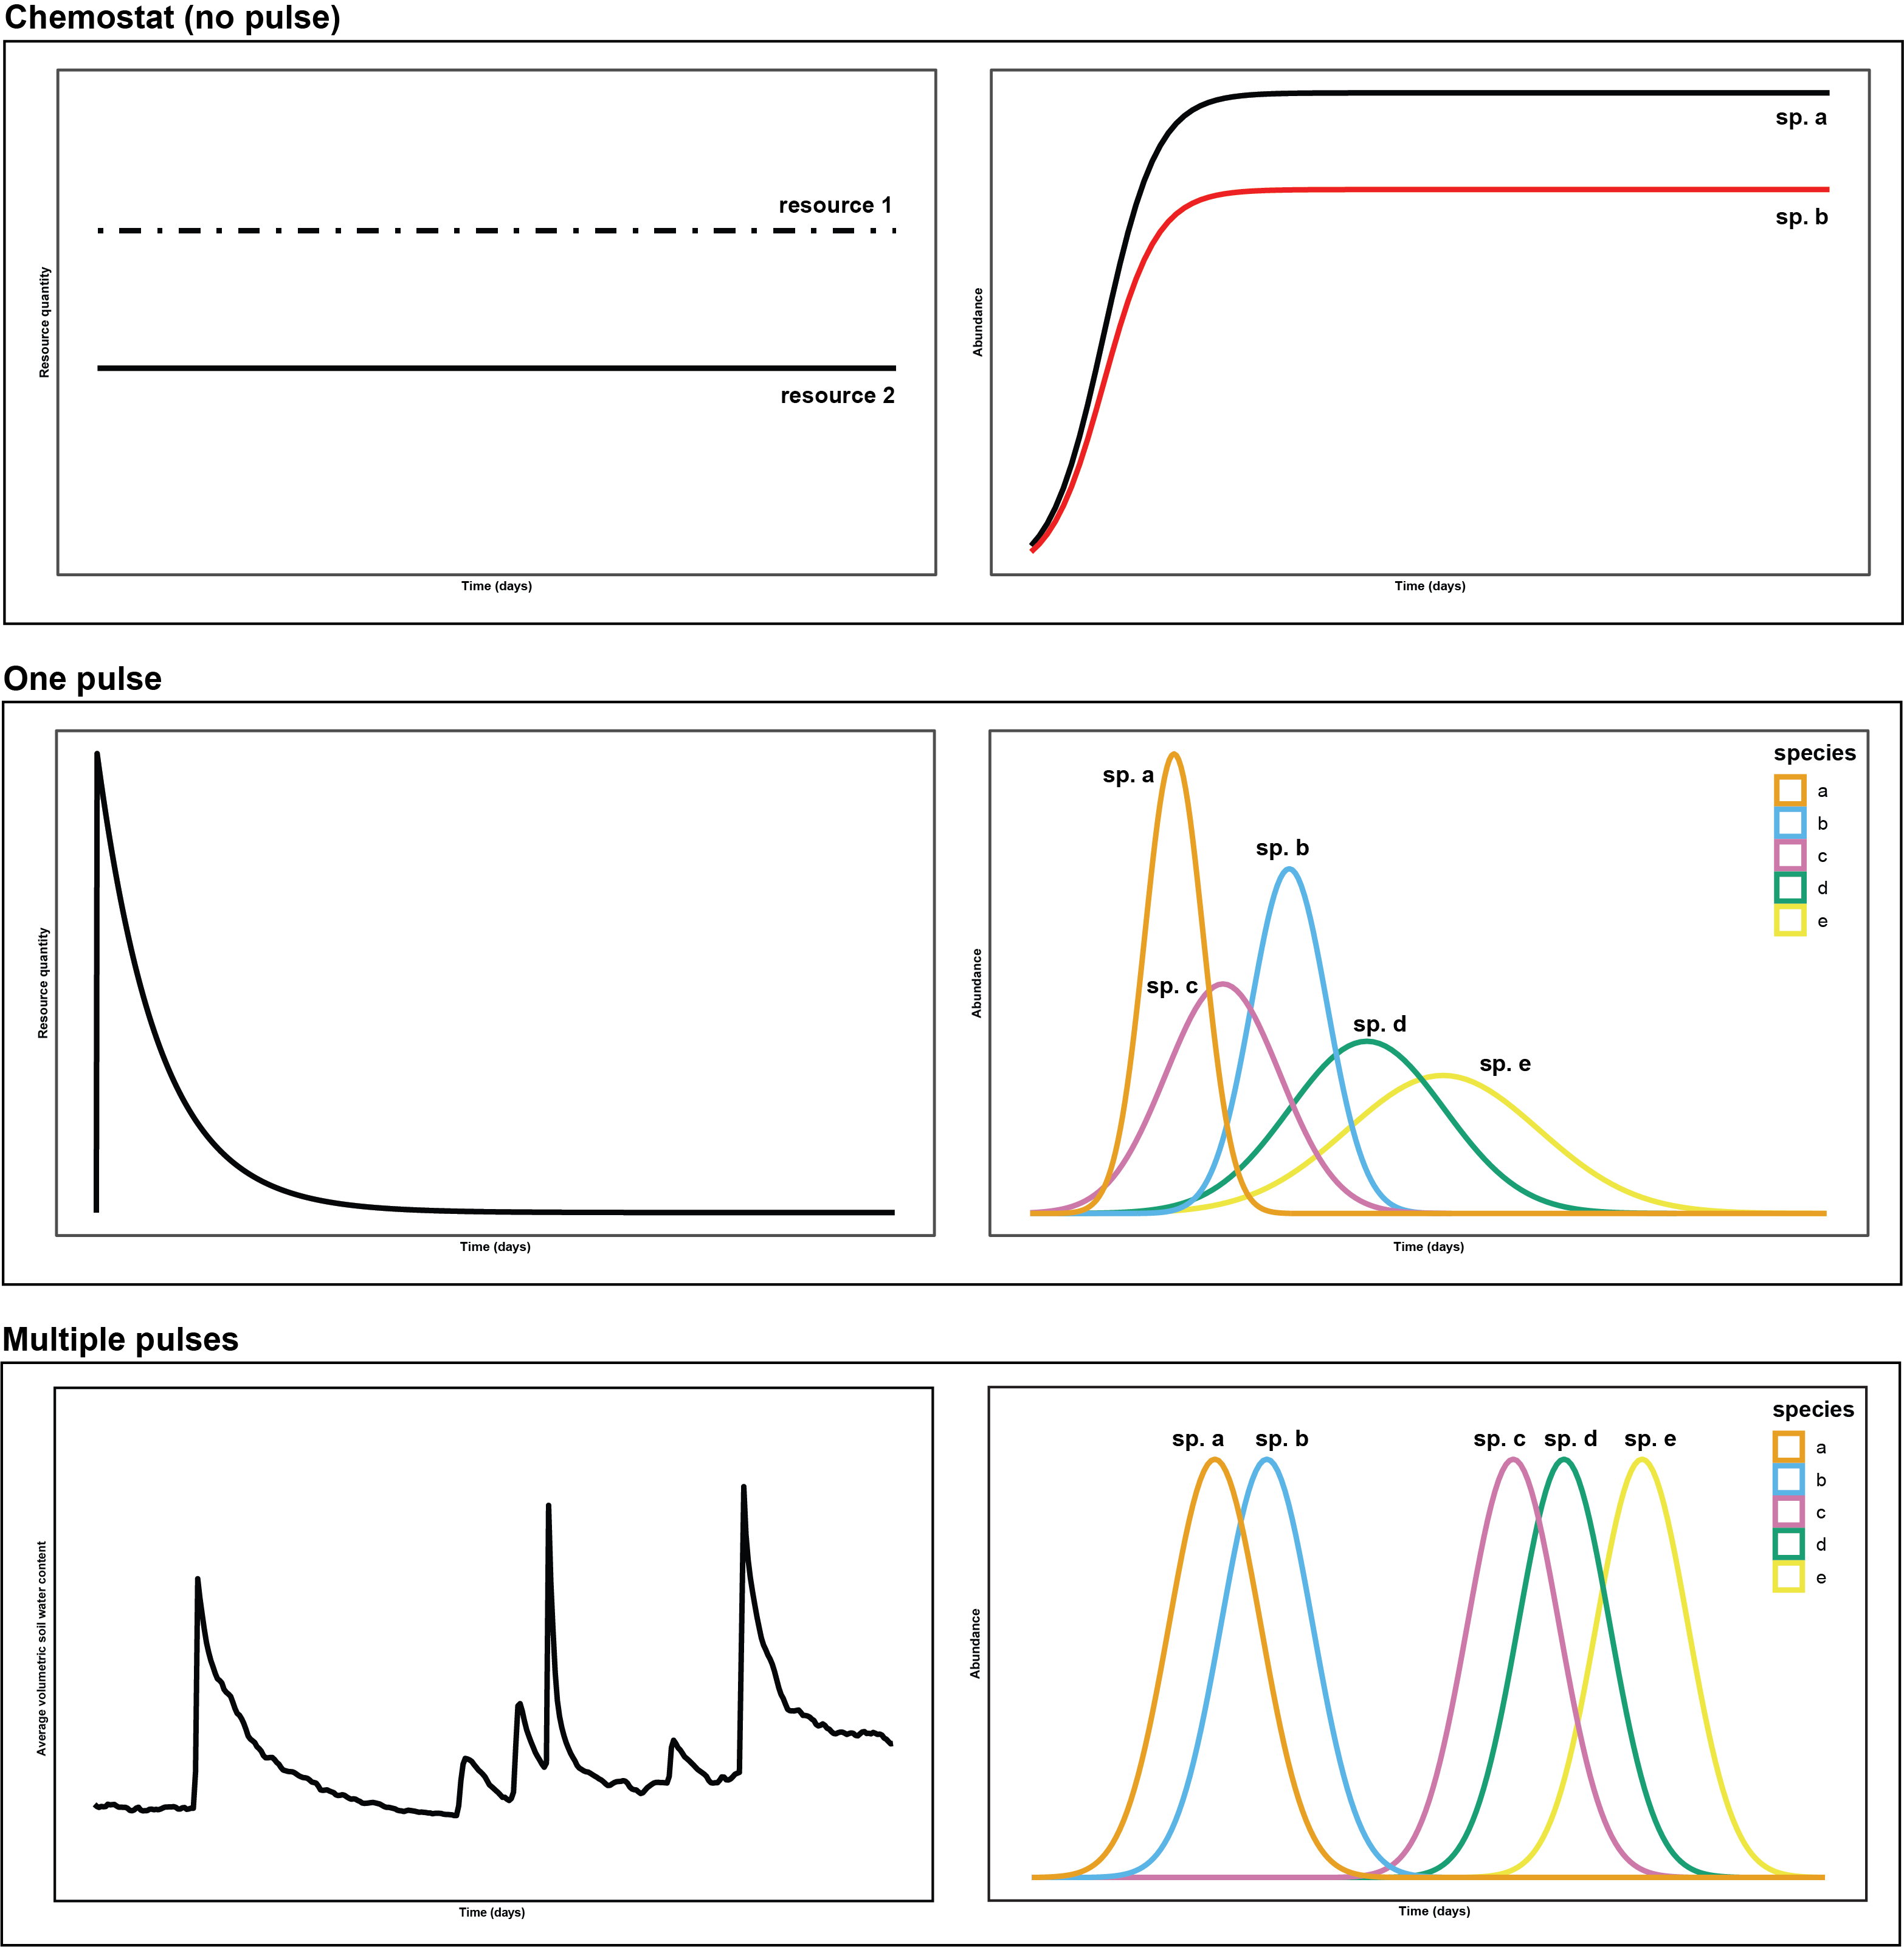
\includegraphics[width=0.8\textwidth]{..//figures/JN_conceptfigs/sixpanel_concept.png}
\caption{Theory suggests resource levels may determine temporal niche space. In a system where resources are constant (top left,, chemostat; species can only coexist if they are each equally good competitors for different resources) species would be expected to show little temporal fluctuations and there would be no real temporal niches. Many models of coexistence today, however, assume a resource pulse that decays (middle, left; e.g., water with evaporative loss, such as in snowpack systems) over time: this resource then sets the temporal window of each season and species compete within it. Most real systems however are more complicated (bottom left, taken from Jornada LTER site 302 showing soil moisture at 10 cm depth over the year) .... [I can work on the caption and figure more if we decide to keep it.]} 
% Evaporating single pulse resource: species may invade only at certain levels of resource (includes snowpack/soil nutrients etc.)
%  Multiple pulses: Some species may persist through whole season or use first or second pulse only
 \label{fig:resource}
\end{figure}


\begin{figure}[h!]
\centering
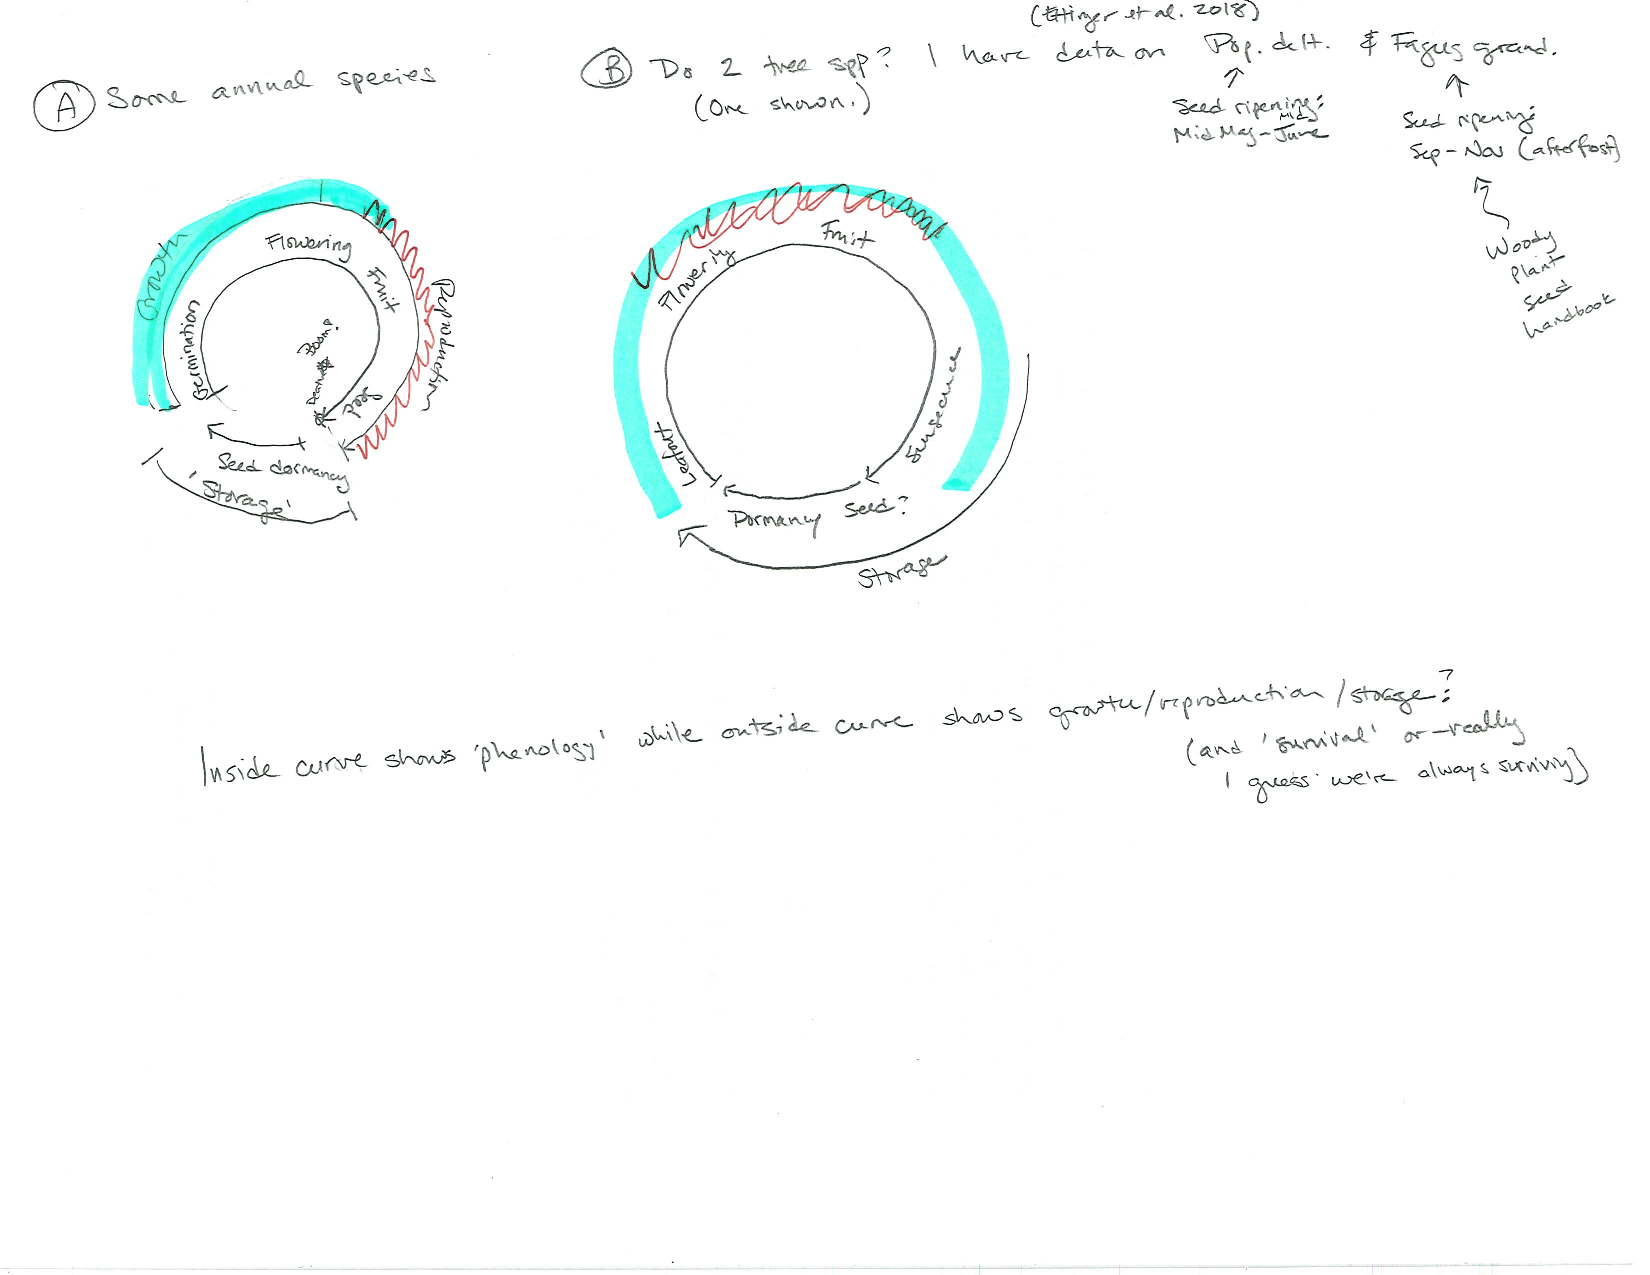
\includegraphics[width=1\textwidth]{..//figures/phenologycircles.pdf}
\caption{Potential figure ... ideally we have data to underlie it (I do for some trees and someone must for Arabidopsis).}
 \label{fig:phenologycircles}
\end{figure}

\clearpage

\begin{figure}[h!]
\centering
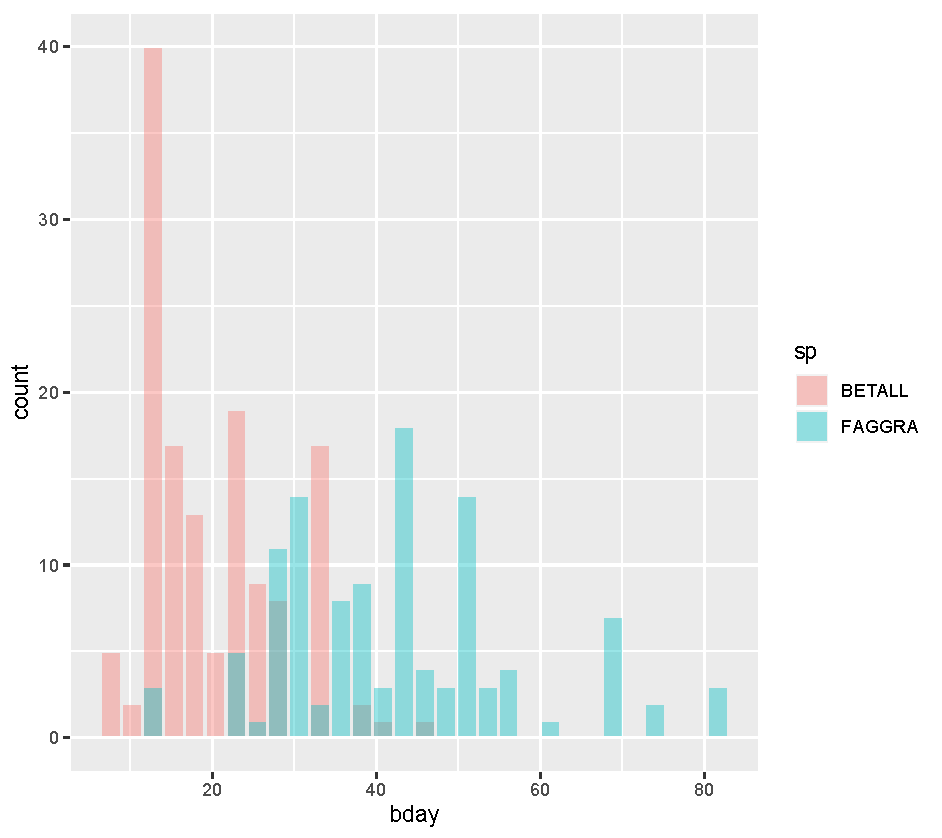
\includegraphics[width=0.6\textwidth]{..//figures/bbdata.pdf}
\caption{Could show budburst data of two species as histogram (shown) and sigmoid (total \% over time, not shown).}
 \label{fig:histsigmoid}
\end{figure}

\clearpage


\begin{figure}[h!]
\centering
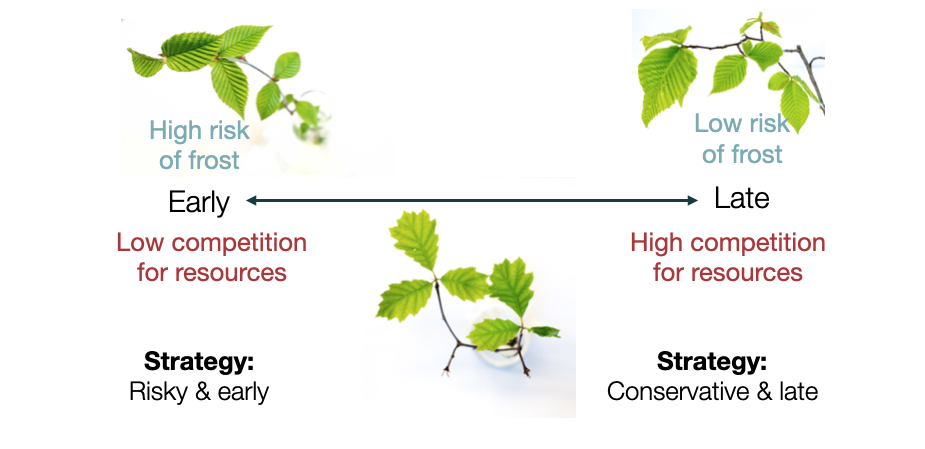
\includegraphics[width=0.8\textwidth]{..//figures/wolkovich_CEFE2023wide_slide.png}
\caption{We could beef this up into a figure about trade-offs? (It's just a slide from a talk now.)}
 \label{fig:seasonaltradeoffs}
\end{figure}



\end{document}
